To assess our models' effectiveness and reduce the potential for overfitting, we implemented a nested cross-validation strategy. The approach is 
designed to accurately gauge the models' capacity to generalize. It features a dual-layer cross-validation system: an outer loop to evaluate the 
models' performance and an inner loop focused on refining hyperparameters. This separation ensures that the evaluation of the models' performance is 
distinct from the optimization process, safeguarding against the models being unduly tailored to a particular dataset and thus avoiding an inflated 
estimation of their performance
~\cite{baumann_baumann_2014}.

\subsubsection*{Nested cross validation}

As illustrated in Fig~\ref{mlPipeline}, our dataset underwent division into $ k = 7 $ segments via stratified sampling for the external loop, ensuring proportional 
representation of the dataset's class distribution within each segment. During each cycle of the external loop, one segment was allocated as the 
testing set to assess model accuracy, while the remaining $ k - 1 $ segments, served as the training set. Encapsulated by this outer loop, an internal 
loop focused on refining the model through hyperparameter adjustments. Here, the training subset was further segmented into $ m = 5 $ portions, again utilizing 
stratified sampling to maintain class distribution consistency. Through this internal loop, a grid search of the hyperparameter space was undertaken, 
employing cross-validation to evaluate the efficacy of each parameter set. The optimal set of hyperparameters was identified based on the best average 
performance across these folds. Moreover, when features for a dataset were not preselected, our pipeline incorporated either the PCA or MRMR feature selection 
algorithm. Subsequently, the ROC AUC score was deployed to quantitatively measure the models' predictive accuracy.

\begin{figure}[!ht]
    \centering
    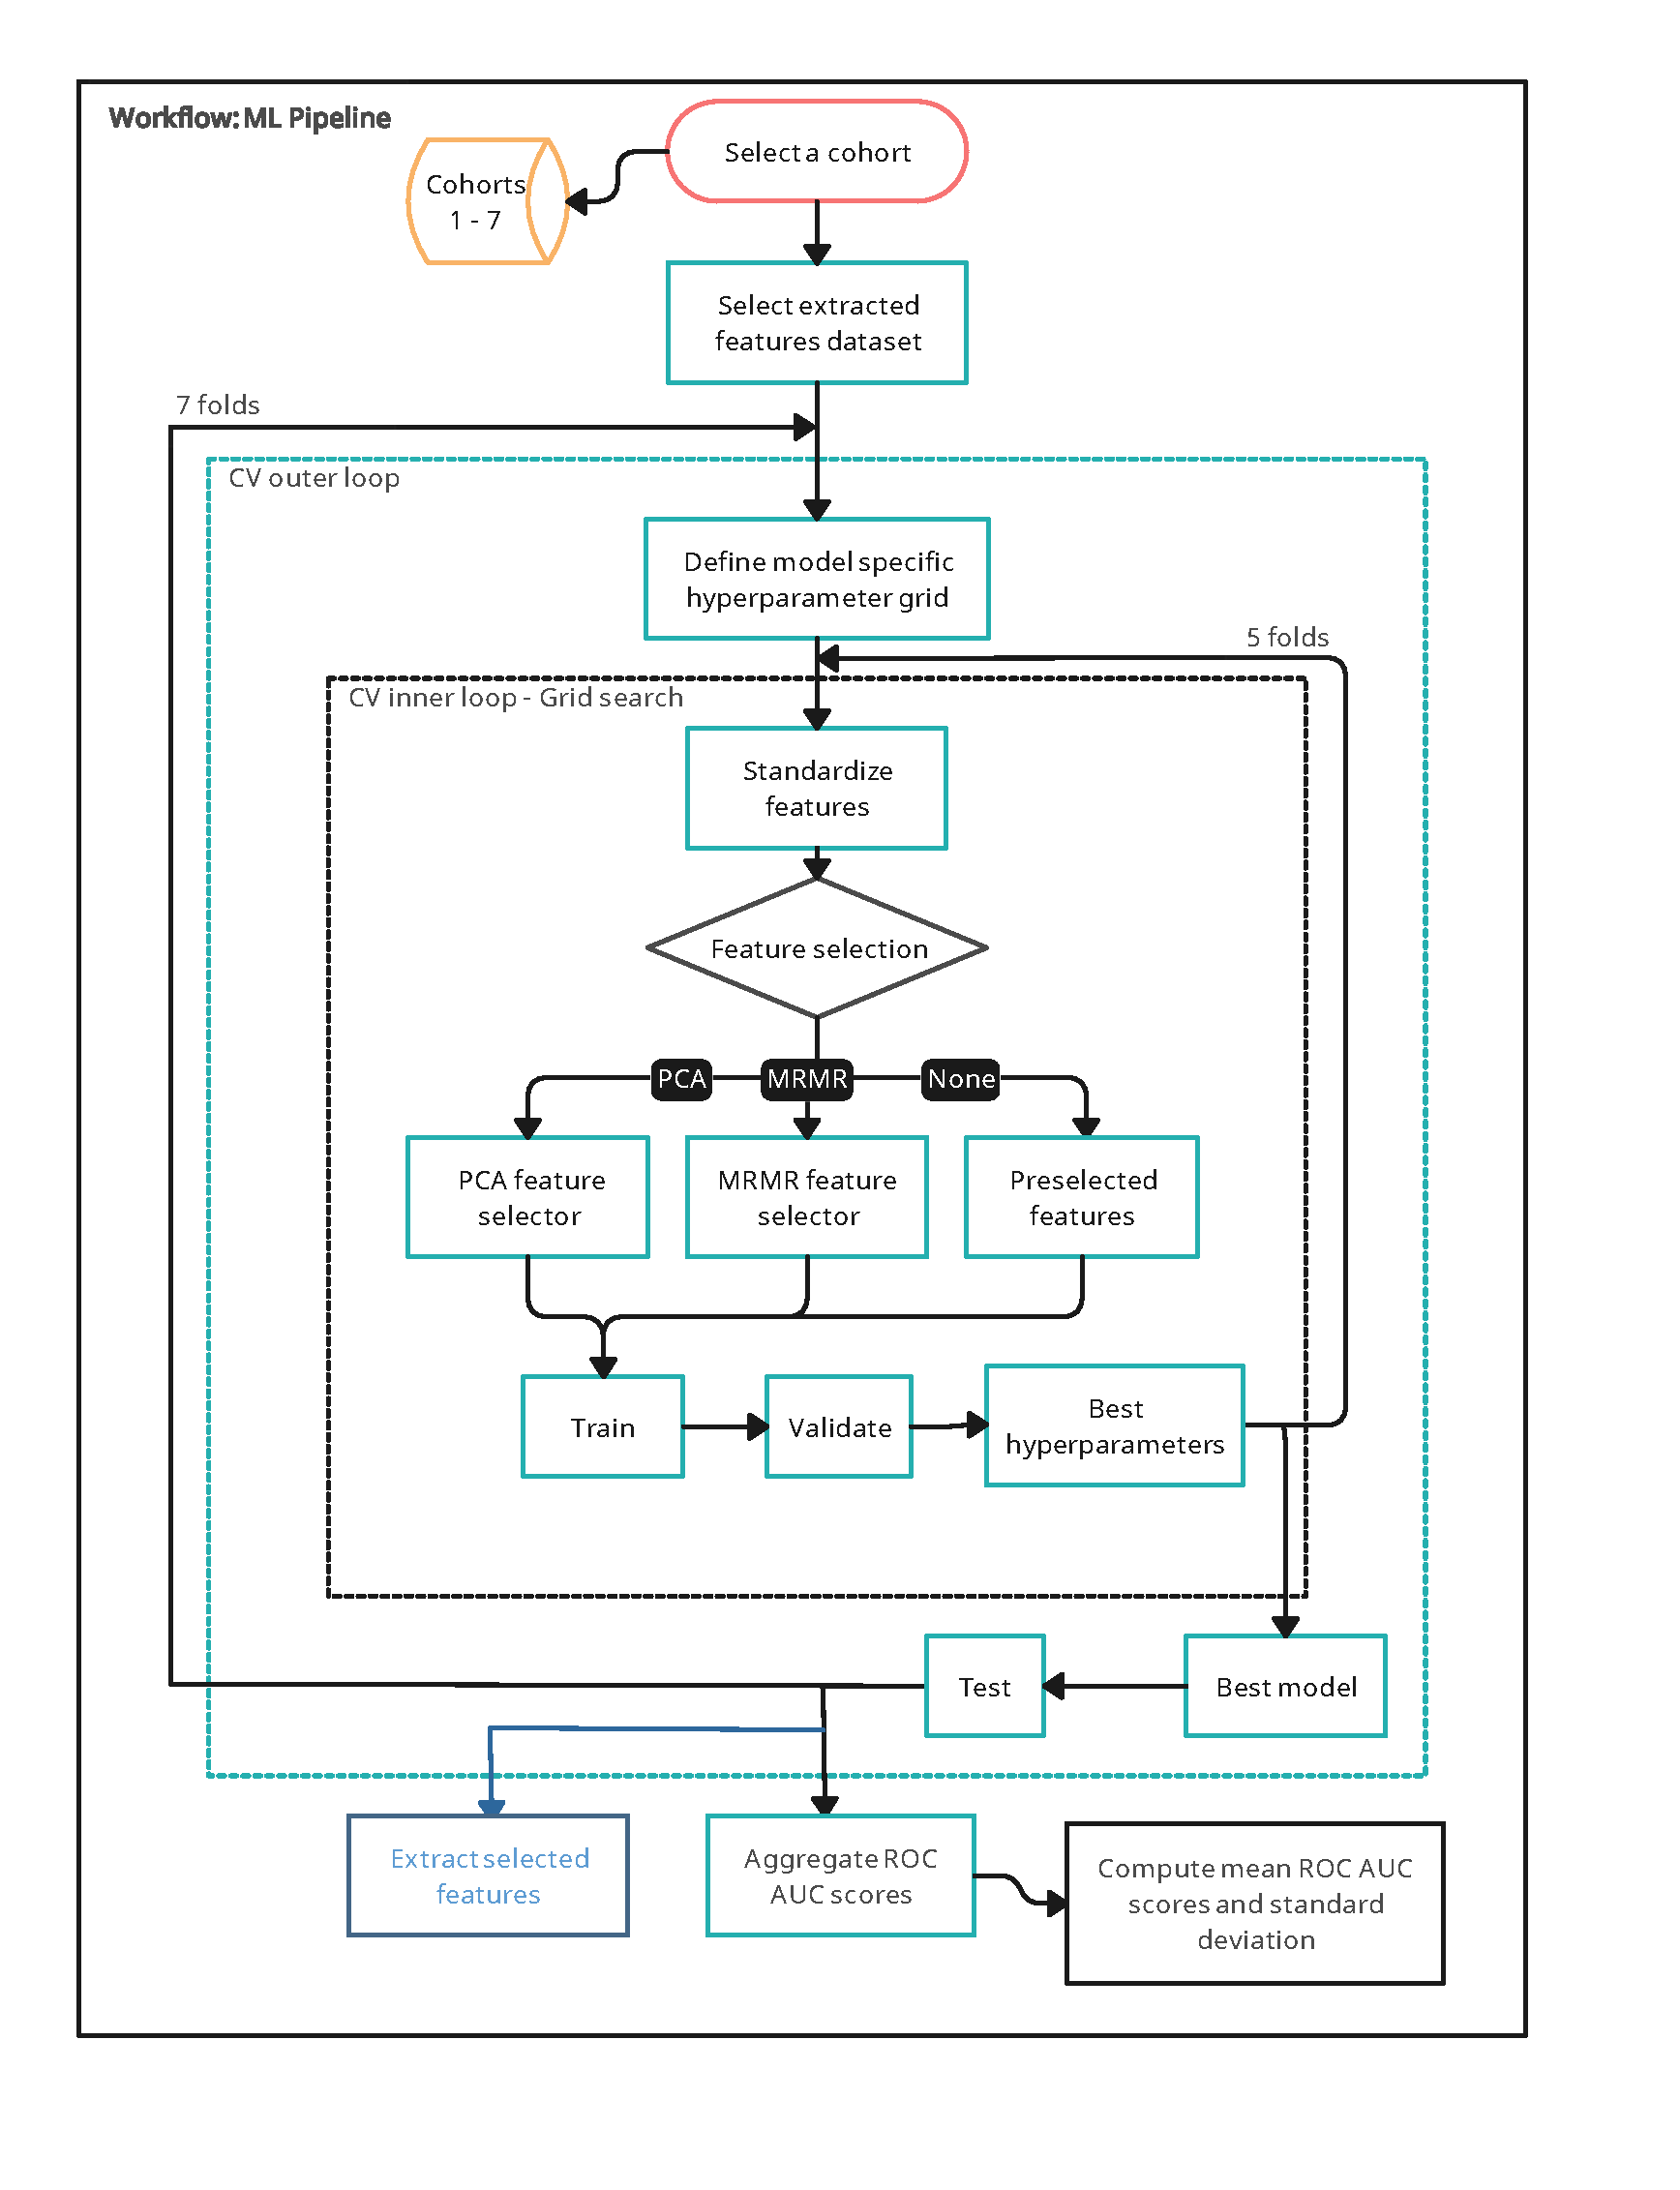
\includegraphics[width=\linewidth]{images/Workflow_ML_pipeline.pdf}
    \caption{{\bf Nested Cross Validation} Model training and evaluation.}
    \label{mlPipeline}
\end{figure}